\usetikzlibrary{arrows.meta,calc,matrix,shapes}
\providecommand{\computer}{%
    
\includegraphics[width=1cm]{../common/Noun_project_216.pdf}
}
\providecommand{\switch}{%
    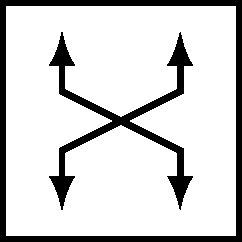
\includegraphics[width=0.9cm]{../common/fig-switch.pdf}
}
\providecommand{\router}{%
    
\includegraphics[width=0.9cm]{../common/fig-router.pdf}
}

\begin{frame}{network and switch tables}
\begin{tikzpicture}
\tikzset{
    computer/.style={inner sep=0mm,outer sep=0mm,execute at begin node={\computer}},
    switch/.style={inner sep=0mm,outer sep=0mm,execute at begin node={\switch}},
    connect/.style={draw,very thick,Latex-Latex},
    connect big/.style={draw,ultra thick,Latex-Latex},
    port/.style={pos=0.95,fill=white,circle,draw,inner sep=0mm},
    port beginning/.style={pos=0.05,fill=white,circle,draw,inner sep=0mm},
    mac label/.style={
        visible on=<2->,draw,fill=white,inner sep=1mm,font=\tiny\tt,
        alt=<2>{text=red,draw=red},
    },
    route table/.style={
        matrix of nodes,ampersand replacement=\&,
        column 1/.style={nodes={draw,thick,text width=2.5cm,font=\tiny\tt,text depth=0mm,minimum height=0.5cm,inner sep=1mm}},
        column 2/.style={nodes={draw,thick,text width=.5cm,font=\small\tt,text depth=0mm,minimum height=0.5cm,inner sep=1mm}},
        row 1/.style={nodes={draw=none,font=\small}},
    }
}
\foreach \x/\d/\mc/\dir in {15/8cm/AA/north,45/3cm/BB/north,90/2cm/CC/north,135/3cm/DD/north,180/4cm/EE/north,300/4cm/FF/south} {
    \node[computer,label={[mac label,]\dir:00:11:22:33:44:\small\mc}] (c-\x) at (\x:\d) {};
}
\node[switch,alt=<4>{fill=red!10}] (s1) at (4,-0.5) {};
\begin{visibleenv}<4->
\matrix[route table,alt=<4>{fill=red!10},anchor=north west] (s1 table) at ([xshift=1cm,yshift=.5cm]s1.north east) {
dst MAC addr \& port \\
00:11:22:33:44:\small AA \& 1 \\
00:11:22:33:44:\small BB \& 2 \\
00:11:22:33:44:\small CC \& 4 \\
00:11:22:33:44:\small DD \& 4 \\
00:11:22:33:44:\small EE \& 4 \\
00:11:22:33:44:\small FF \& 3 \\
};
\draw[dotted,thick] (s1.north east) -- (s1 table-2-1.north west);
\draw[dotted,thick] (s1.south east) -- (s1 table-7-1.south west);
\end{visibleenv}
\node[switch,alt=<3>{fill=red!10}] (s2) at (-1,0.5) {};
\begin{visibleenv}<3->
\matrix[route table,alt=<3>{fill=red!10},anchor=north east] (s2 table) at ([xshift=2cm]s2.south west) {
dst MAC addr \& port \\
00:11:22:33:44:\small AA \& 1 \\
00:11:22:33:44:\small BB \& 1 \\
00:11:22:33:44:\small CC \& 2 \\
00:11:22:33:44:\small DD \& 3 \\
00:11:22:33:44:\small EE \& 4 \\
00:11:22:33:44:\small FF \& 2 \\
};
\draw[dotted,thick] (s2.south east) -- (s2 table-2-2.north east);
\draw[dotted,thick] (s2.south west) -- (s2 table-2-1.north west);
\end{visibleenv}
\draw[connect] (c-15) -- (s1) node[port] {1};
\draw[connect] (c-45) -- (s1) node[port] {2};
\draw[connect] (c-300) -- (s1) node[port] {3};
\draw[connect] (c-90) -- (s2) node[port] {2};
\draw[connect] (c-135) -- (s2) node[port] {3};
\draw[connect] (c-180) -- (s2) node[port] {4};
\draw[connect big] (s1) -- (s2) node[port beginning] {4} node [port] {1};
\end{tikzpicture}
\end{frame}

\begin{frame}{constructing switch tables}
    \begin{itemize}
    \item could have system administrator input these by hand
        \begin{itemize}
        \item through an SSH-like interface, probably
        \end{itemize}
    \item works, but error-prone, hard to change, etc.
    \vspace{.5cm}
    \item<2-> alternative: switch should figure it out
    \end{itemize}
\end{frame}

\begin{frame}{MAC learning}
\begin{tikzpicture}
\tikzset{
    route table/.style={
        matrix of nodes,ampersand replacement=\&,
        column 1/.style={nodes={draw,thick,text width=2.5cm,font=\tiny\tt,text depth=1mm,text height=3.5mm,minimum height=0.6cm,inner sep=1mm}},
        column 2/.style={nodes={draw,thick,text width=1cm,font=\small\tt,text depth=1mm,text height=3.5mm,minimum height=0.6cm,inner sep=1mm}},
        row 1/.style={nodes={draw=none,font=\small}},
    }
}
\matrix[label={north:forwarding table},route table,draw,very thick,anchor=north east] (table) {
dst MAC addr \& port \\
|[alt={<5,7>{fill=red!10}}]| \alt<5->{00:11:22:33:44:AA}{~}
    \& |[alt={<5,7>{fill=red!10}}]| \alt<5->{2}{~} ~ \\
|[alt={<8>{fill=red!10}}]| \alt<8->{00:11:22:33:44:FF}{~}
    \& |[alt={<8>{fill=red!10}}]| \alt<8->{3}{~} ~ \\
~ \& ~ \\
~ \& ~ \\
~ \& ~ \\
~ \& ~ \\
|[alt={<2,4>{fill=red!10}}]|  \alt<2->{(default)}{~} 
    \& |[alt={<2,4>{fill=red!10}}]| \alt<2->{ALL*}{~} \\
};
\begin{visibleenv}<3->
\matrix[
    draw,very thick,label={north:incoming frame 1},anchor=north west,tight matrix,
    nodes={text width=8cm,font=\small}
] (pkt 1) at ([xshift=1cm]table.north east) {
    input port=\myemph<5>{2}, output port = \alt<4->{\myemph<4>{all but 2}}{\myemph<3>{???}} \\
    data = {
\begin{tabular}{l}
src=\tt \myemph<5>{00:11:22:33:44:AA} \\ dst=\tt \myemph<2>{00:11:22:33:44:FF} \\
type = IPV4  \\ data = \tt33 45 43 42 \ldots \\
\end{tabular}
} \\
};
\end{visibleenv}
\begin{visibleenv}<6->
\matrix[
    draw,very thick,label={north:incoming frame 2},anchor=north west,tight matrix,
    nodes={text width=8cm,font=\small}
] (pkt 2) at ([yshift=-1cm]pkt 1.south west) {
    input port=\myemph<8>{3}, output port = \alt<7->{\myemph<7>{2}}{???} \\
    data = {
\begin{tabular}{l}
src=\tt \myemph<8>{00:11:22:33:44:FF} \\ dst=\tt \myemph<7>{00:11:22:33:44:AA} \\
type = IPV4  \\ data = \tt34 45 43 42 \ldots \\
\end{tabular}
} \\
};
\end{visibleenv}
\end{tikzpicture}
\end{frame}

% FIXME: picture of network with switch ports labeled
    % FIXME: picture of ideal mac_dst_exact tables for it

